% Written by paper_style.save; edit the figure code, not this file.
% Needs \usepackage{graphicx,amssymb,textcomp} in the preamble.
\begin{figure*}[t]
  \centering
  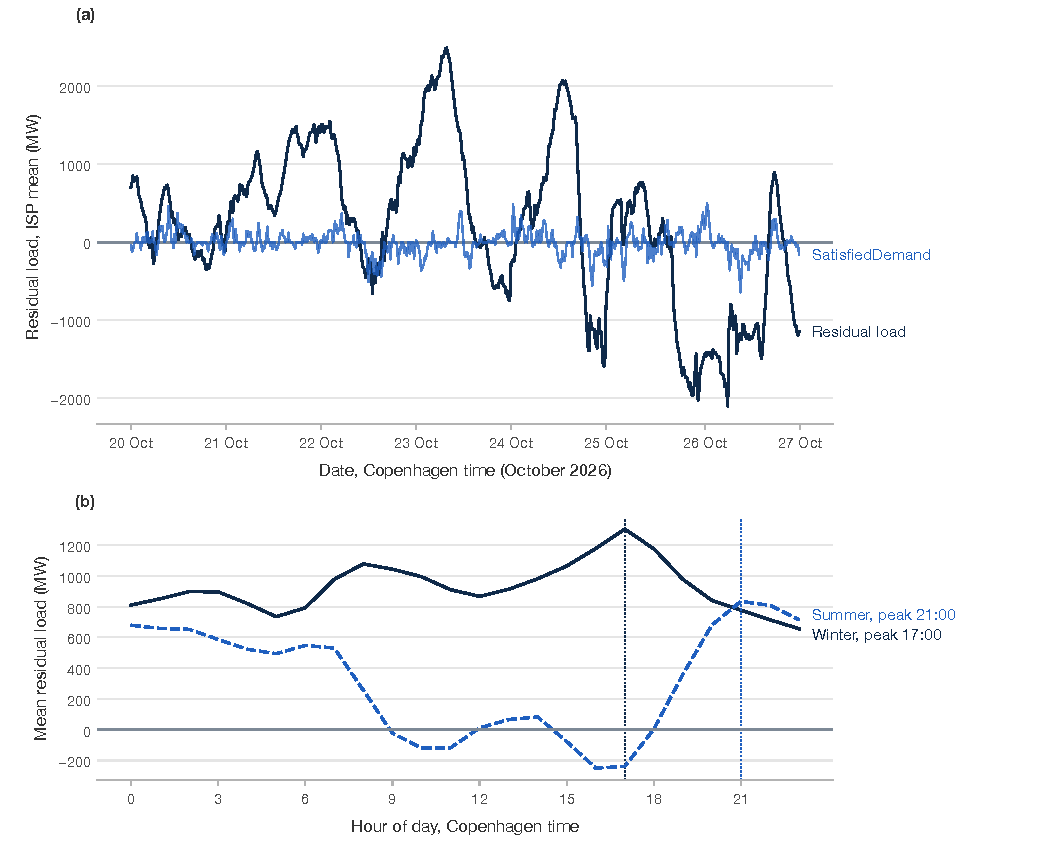
\includegraphics[width=\linewidth]{residual_load.pdf}
  \caption{DK1 residual load peaks at 17:00 in winter and 21:00 in summer. (a) DK1 residual load, 20-26 Oct 2026, with the imbalance target (SatisfiedDemand) for scale, Copenhagen time. (b) Mean residual load by Copenhagen hour, winter (Dec-Feb) against summer (Jun-Aug), from the first prints since 1 Oct 2025; each season's peak hour (dotted) is read from the data, not assumed. Residual load = demand minus wind minus solar; thermal = plants \textless{}100 MW + 100 MW or larger; net import = six exchanges, + = import. Units: MW; quarter-hourly. Source: Energinet, Energi Data Service (ElectricityProdex5MinRealtime, first prints); CC BY 4.0; as of 2026-10-29.}
  \label{fig:residual-load}
\end{figure*}
